% ========================================
% template.tex
% A single-file template that merges "reedthesis"-style macros
% into a standard book-based template for use with bookdown.
% ========================================
\documentclass[12pt,twoside]{book}

\usepackage{color}
\usepackage{fancyvrb}
\newcommand{\VerbBar}{|}
\newcommand{\VERB}{\Verb[commandchars=\\\{\}]}
\DefineVerbatimEnvironment{Highlighting}{Verbatim}{commandchars=\\\{\}}
% Add ',fontsize=\small' for more characters per line
\usepackage{framed}
\definecolor{shadecolor}{RGB}{248,248,248}
\newenvironment{Shaded}{\begin{snugshade}}{\end{snugshade}}
\newcommand{\AlertTok}[1]{\textcolor[rgb]{0.94,0.16,0.16}{#1}}
\newcommand{\AnnotationTok}[1]{\textcolor[rgb]{0.56,0.35,0.01}{\textbf{\textit{#1}}}}
\newcommand{\AttributeTok}[1]{\textcolor[rgb]{0.13,0.29,0.53}{#1}}
\newcommand{\BaseNTok}[1]{\textcolor[rgb]{0.00,0.00,0.81}{#1}}
\newcommand{\BuiltInTok}[1]{#1}
\newcommand{\CharTok}[1]{\textcolor[rgb]{0.31,0.60,0.02}{#1}}
\newcommand{\CommentTok}[1]{\textcolor[rgb]{0.56,0.35,0.01}{\textit{#1}}}
\newcommand{\CommentVarTok}[1]{\textcolor[rgb]{0.56,0.35,0.01}{\textbf{\textit{#1}}}}
\newcommand{\ConstantTok}[1]{\textcolor[rgb]{0.56,0.35,0.01}{#1}}
\newcommand{\ControlFlowTok}[1]{\textcolor[rgb]{0.13,0.29,0.53}{\textbf{#1}}}
\newcommand{\DataTypeTok}[1]{\textcolor[rgb]{0.13,0.29,0.53}{#1}}
\newcommand{\DecValTok}[1]{\textcolor[rgb]{0.00,0.00,0.81}{#1}}
\newcommand{\DocumentationTok}[1]{\textcolor[rgb]{0.56,0.35,0.01}{\textbf{\textit{#1}}}}
\newcommand{\ErrorTok}[1]{\textcolor[rgb]{0.64,0.00,0.00}{\textbf{#1}}}
\newcommand{\ExtensionTok}[1]{#1}
\newcommand{\FloatTok}[1]{\textcolor[rgb]{0.00,0.00,0.81}{#1}}
\newcommand{\FunctionTok}[1]{\textcolor[rgb]{0.13,0.29,0.53}{\textbf{#1}}}
\newcommand{\ImportTok}[1]{#1}
\newcommand{\InformationTok}[1]{\textcolor[rgb]{0.56,0.35,0.01}{\textbf{\textit{#1}}}}
\newcommand{\KeywordTok}[1]{\textcolor[rgb]{0.13,0.29,0.53}{\textbf{#1}}}
\newcommand{\NormalTok}[1]{#1}
\newcommand{\OperatorTok}[1]{\textcolor[rgb]{0.81,0.36,0.00}{\textbf{#1}}}
\newcommand{\OtherTok}[1]{\textcolor[rgb]{0.56,0.35,0.01}{#1}}
\newcommand{\PreprocessorTok}[1]{\textcolor[rgb]{0.56,0.35,0.01}{\textit{#1}}}
\newcommand{\RegionMarkerTok}[1]{#1}
\newcommand{\SpecialCharTok}[1]{\textcolor[rgb]{0.81,0.36,0.00}{\textbf{#1}}}
\newcommand{\SpecialStringTok}[1]{\textcolor[rgb]{0.31,0.60,0.02}{#1}}
\newcommand{\StringTok}[1]{\textcolor[rgb]{0.31,0.60,0.02}{#1}}
\newcommand{\VariableTok}[1]{\textcolor[rgb]{0.00,0.00,0.00}{#1}}
\newcommand{\VerbatimStringTok}[1]{\textcolor[rgb]{0.31,0.60,0.02}{#1}}
\newcommand{\WarningTok}[1]{\textcolor[rgb]{0.56,0.35,0.01}{\textbf{\textit{#1}}}}
% ------------------------------------------------
% PACKAGES
% ------------------------------------------------
\usepackage{amsmath,amssymb,amsthm}
\usepackage{longtable,booktabs,array}
\usepackage{graphicx}
\usepackage{hyperref}
\usepackage{xcolor}
\usepackage{fancyhdr}
\usepackage{lmodern}
\usepackage{float}
\usepackage{rotating}
\usepackage{fancyvrb} % for nicer verbatim
\usepackage[round]{natbib}
\bibliographystyle{abbrvnat}

% For cross-referencing sections with auto-labeled references

% --- Page geometry / margins (if not using geometry in YAML) ---
  \usepackage[margin=1in]{geometry}

\providecommand{\tightlist}{%
  \setlength{\itemsep}{0pt}\setlength{\parskip}{0pt}}
% ------------------------------------------------
% THESIS/DISSERTATION-SPECIFIC MACROS
% ------------------------------------------------
\makeatletter
\newcommand{\degree}[1]{\def\@degree{#1}}
\newcommand{\institution}[1]{\def\@institution{#1}}
\newcommand{\division}[1]{\def\@division{#1}}
\newcommand{\department}[1]{\def\@department{#1}}
\newcommand{\advisor}[1]{\def\@advisor{#1}}
\newcommand{\altadvisor}[1]{\def\@altadvisor{#1} \@altadvisortrue}
\newcommand{\startquote}[1]{\def\@startquote{#1}}


% Defaults if user doesn't provide them via YAML
\def\@degree{PhD}
\def\@institution{My University}
\def\@division{Science Division}
\def\@department{Department Name}
\def\@advisor{Advisor Name}
\def\@altadvisor{}
\def\@startquote{}

% Pandoc will pass these from YAML front matter if present
  \degree{Doktors der Naturwissenschaften (Dr.~rer. nat.)}
  \institution{der Brandenburgischen Technischen Universität Cottbus-Senftenberg}
  \division{Von der Fakultät für Umwelt und Naturwissenschaften}
  \advisor{M Hupfer}
  \department{Leibniz-Institut für Gewässerökologie und Binnenfischerei}
  \startquote{\emph{Planet Earth is blue}\\
\emph{and there's nothing we can do}\\
\textbf{David Bowie}}

% Title, author, date from YAML
  \title{Impacts of Sulfate Reduction on Phosphorus Cycling: Stability of Vivianite in Lake Sediments}

  \author{Harm Noël van Kuppevelt}

  \date{May 2025}

% ------------------------------------------------
% HEADERS/FOOTERS
% ------------------------------------------------
\pagestyle{fancy}
\fancyhf{}
\fancyhead[LE,RO]{\thepage}
\fancyhead[LO]{\slshape \nouppercase \rightmark}
\fancyhead[RE]{\slshape \nouppercase \leftmark}

% ------------------------------------------------
% FRONTMATTER / ENVIRONMENTS
% ------------------------------------------------
\newenvironment{preface}{
  \chapter*{Preface}
  \addcontentsline{toc}{chapter}{Preface}
}{\clearpage}

\newenvironment{acknowledgements}{
  \chapter*{Acknowledgements}
  \addcontentsline{toc}{chapter}{Acknowledgements}
}{\clearpage}

\newenvironment{summary}{
  \chapter*{Summary}
  \addcontentsline{toc}{chapter}{Summary}
}{\clearpage}

\newenvironment{zusammenfassung}{
  \chapter*{Zusammenfassung}
  \addcontentsline{toc}{chapter}{Zusammenfassung}
}{\clearpage}

% ------------------------------------------------
% BEGIN DOCUMENT
% ------------------------------------------------
\begin{document}

% -----------------------------------------------
% CUSTOM TITLE PAGE (Mimicking "reedthesis" style)
% -----------------------------------------------
  \thispagestyle{empty}
  \begin{titlepage}
    \centering
    \vspace*{2cm}
    {\Large \textbf{\@title}\par}
    \vspace{1cm}
    {\large \@division \\
    \@institution \\
    for the degree of \\
    \@degree \\}
    \vspace{2cm}
    {\large \@author \\
    \@department\par}
    \vspace{1.5cm}
    Advisor: \@advisor \\
        \vfill
    {\large \@date}
  \end{titlepage}
  \cleardoublepage

% If a "quote" was provided, show it on a separate page

  \thispagestyle{empty}
  \begin{flushright}
    \vspace*{4cm}
    \emph{\@startquote}
  \end{flushright}
  \cleardoublepage

  \makeatother
% Use frontmatter to get roman-numbered pages here
\frontmatter
\pagestyle{empty}

% If you want an optional "preface" environment:


  \setcounter{tocdepth}{3}
  \tableofcontents
  \clearpage

  \begin{summary}
  This is the document

  \par

  Second paragraph of abstract starts here.
  \end{summary}

  \begin{zusammenfassung}
  This is the abstract in German

  \par

  Second paragraph of abstract starts here.
  \end{zusammenfassung}

% Start mainmatter for normal arabic page numbering
\mainmatter
\pagestyle{fancy}

% -----------------------------------------------
% HERE IS THE BOOK CONTENT INJECTED BY bookdown
% -----------------------------------------------
\chapter{Introduction}\label{Intro}

Per Morgen- SEM-EDS
SDU lab technicians
Aarhus people

\section{The Phosphorus problem}\label{the-phosphorus-problem}

The emergence of humans on earth was followed by unprecedented changes in the Earths environment and disruption of the vital biogeochemical cycles underpinning the regenerative nature that characterized the climatologically stable Holocene epoch. As a species that can recognize the importance of live and its essential building blocks, we bear the responsibility of a fair and sustainable distribution of the earths resources. Unfortunately, externalizing impacts in favor of short-term profit has become humanities predominant mode of operation. The limits of regeneration are increasingly crossed, as described by the planetary boundary framework (\citep{Richardson2023}). One of the transgressed boundaries is that of Phosphorus (P). The geological P cycle, P weathering from rocks flow in the ocean where it precipitates again, is a slow process, and many ecosystems are P limited. As an essential building block of life, P is recycled efficiently in natural ecosystems. Since the green revolution, agriculture is increasingly dependent on the use of fertilizer derived from phosphate rock \citep{Ashley2011}. This has broken the P cycle, instead forming a linear process with major implications at both ends of the chain \citep{Cordell2010}. On one end, food production has become dependent on a finite reservoir of phosphate rock, while accumulation of P in freshwater ecosystems causes wide spread ecological damage at the other end (Fig. \ref{fig:pcycle}). Harmful algae blooms through eutrophication threaten water quality and many related ecosystem services \citep{Ansari2014}. Closing the P cycle requires not just the reuse of P in agriculture, but also the restoration of lake ecosystems.

\begin{figure}

{\centering \includegraphics[width=1\linewidth]{figure/pcyclelinear} 

}

\caption{Top: geological P cycle. Bottom: Unstustainable P use. A finite resource of phosphate rock is used in agriculture and ends up in aquatic ecosystems, where it causes ecological damage.}\label{fig:pcycle}
\end{figure}

\section{Phosphorus cycling in freshwater sediments}\label{phosphorus-cycling-in-freshwater-sediments}

Talk about all the different forms P enters the sediment, and the early diagenesis.

The retention of P in sediments occurs through its binding to the solid phase via biological and chemical precipitation \citep{Boers1998, OConnell2020, Parsons2017}. Burial P pools accumulate in sediment following years of nutrient enrichment. The speciation of sediment P is highly dependent on lake conditions and undergoes significant changes during early diagenesis, where remobilisation of labile forms of P occurs, whereas only the stable forms of solid-bound P are buried long-term (Boers et al., 1998; Emerson, 1976). Initially, the sedimentation of P incorporated into organic matter (OM) by primary producers is an important influx of P to lake sediments, especially in eutrophic lakes. However, the long-term burial of OM-bound P is constrained by remineralisation processes in the sediment (Boers et al., 1998). Secondly, P can adsorb to iron (Fe) hydroxides \citep{Gunnars2002} and bind to OM to form organic Fe-P complexes (Fe(III)-OM-P) (Schwertmann and Murad, 1988). The precipitation of these ferric iron-bound P forms (Fe(III)-P) can be a major internal sink of P in lakes with naturally high Fe content (Hupfer and Lewandowski, 2008; Reitzel et al., 2005) or those artificially treated with Fe (Kleeberg et al., 2012; Münch et al., 2024). Under the reducing conditions induced by organic matter decomposition in the sediment, Fe(III) is reduced to Fe(II), leading to the release of bound P and preventing the long-term burial of Fe(III)-bound P. However, P can be sequestered long-term in the form of the Fe(II) mineral vivianite (Fe(II)3(PO4)2·8H2O) (Rothe et al., 2016), which has been identified as a major form of burial P in eutrophic, high-Fe, and nonsulphidic freshwater systems (Dijkstra et al., 2018; Kubeneck et al., 2021; O'Connell et al., 2015; Rothe, 2016).

\section{Sulfur biogeochemistry}\label{sulfur-biogeochemistry}

Basically summarize \citet{Zak2021}.

-- This analysis revealed three main clusters of research: one focused on biogeochemical processes in wetlands and lakes (emphasizing carbon, nitrogen, and methane dynamics), another on the ecotoxicological effects of sulfate (with emphasis on eutrophication and toxicity in various species), and a third on bioremediation approaches to mitigate sulfate pollution.

\begin{enumerate}
\def\labelenumi{\arabic{enumi}.}
\setcounter{enumi}{2}
\tightlist
\item
  Impact on Biogeochemical Cycles
  • Carbon Cycle:
  -- Elevated sulfate levels can alter primary production, organic matter decomposition, and the overall balance between methane (CH₄) and carbon dioxide (CO₂) production.
  -- Under anaerobic conditions, sulfate-reducing bacteria (SRB) become energetically favored over methanogens, shifting the electron flow from methanogenesis (which produces CH₄) to sulfate reduction (producing CO₂).
  -- This transition can result in a diversion of carbon flow, potentially enhancing overall carbon mineralization rates and influencing greenhouse gas emissions.
\end{enumerate}

• Phosphorus Cycle:
-- Sulfate reduction in sediments can lead to the production of sulfide, which in turn affects iron chemistry.
-- The reduction of Fe(III) compounds and subsequent precipitation of iron sulfides can liberate phosphate from sediments, thereby increasing its availability in the water column---a process sometimes referred to as ``internal eutrophication.''
-- This mechanism is especially critical in systems with high iron-bound phosphorus, where changes in the Fe:PO₄³⁻ ratio can trigger a net release of phosphorus into the water.

\begin{enumerate}
\def\labelenumi{\arabic{enumi}.}
\setcounter{enumi}{3}
\tightlist
\item
  Ecotoxicological Effects and Human Health Implications
  • Toxicity to Aquatic Organisms:
  -- Although sulfate itself is often considered one of the less toxic major ions, its presence can induce osmotic stress. The paper details that many freshwater species (e.g., invertebrates, certain fish, amphibians, and aquatic plants) exhibit reduced physiological performance at elevated sulfate concentrations.
  -- Sensitivity to sulfate often depends on water chemistry; for instance, higher water hardness and the presence of chloride can mitigate some toxic effects, whereas soft water systems are more vulnerable.
\end{enumerate}

• Role of Sulfide:
-- The ecotoxicological concern is compounded by the fact that sulfate reduction yields hydrogen sulfide (H₂S), a compound known for its high toxicity to aquatic life.
-- Elevated levels of sulfide can affect respiration, growth, and reproduction across a range of organisms, thereby impacting community structure and ecosystem services.

• Human Health Considerations:
-- The review also touches on potential implications for human health, particularly in relation to drinking water quality.
-- Many freshwater sources used for human consumption can be affected by sulfate levels, which in turn are regulated by environmental quality standards that consider both sulfate and its metabolites.

\begin{enumerate}
\def\labelenumi{\arabic{enumi}.}
\setcounter{enumi}{4}
\tightlist
\item
  Bioremediation Strategies
  • Mitigation Approaches:
  -- The paper reviews a variety of bioremediation techniques aimed at reducing sulfate loads in contaminated water bodies.
  -- Constructed wetlands, permeable reactive barriers, and bioreactors are evaluated, with reported removal efficiencies ranging from 0\% to 70\%.
  -- While promising, these technologies are highly variable in performance due to factors such as hydraulic residence time, microbial community composition, and the specific chemical environment.
\end{enumerate}

• Research Gaps and Future Directions:
-- The authors emphasize that there is a pressing need for more field-scale studies to better understand the long-term trends and spatial dynamics of sulfate pollution.
-- They call for further research into the interactions between sulfate pollution, climate change, and land-use practices, as well as the development of more robust and scalable bioremediation systems.

\begin{enumerate}
\def\labelenumi{\arabic{enumi}.}
\setcounter{enumi}{5}
\tightlist
\item
  Conclusions
  • The review concludes that the global perturbation of the sulfur cycle---driven by both legacy pollution and ongoing anthropogenic activities---is likely to have widespread and long-lasting effects on freshwater ecosystems.
  • The interplay between sulfate and major biogeochemical cycles is complex, influencing greenhouse gas emissions, nutrient dynamics, and ecological health.
  • There is a critical need for integrative, interdisciplinary research to refine our understanding of these processes and to develop effective mitigation strategies that protect both ecosystem function and human health.
\end{enumerate}

This detailed synthesis provides a thorough overview suitable for researchers interested in the environmental chemistry, ecological impacts, and remediation of sulfate pollution in freshwater systems. For further details, please refer to the full article by Zak et al.~(2020) in Earth-Science Reviews.

\subsection{Sources and sinks for sulfur}\label{sources-and-sinks-for-sulfur}

Sources and Trends of Sulfate in Freshwaters
• Natural versus Anthropogenic Inputs:
-- The review begins by distinguishing between natural sulfate sources---such as mineral weathering, volcanic emissions, sea spray aerosols, and the oxidation of naturally occurring sulphides---and anthropogenic sources.
-- Anthropogenic activities such as industrial emissions, acid mine drainage (AMD), wetland drainage, agricultural fertilization, and even historical practices (e.g., fertilization with sulfate-containing superphosphate) have substantially increased sulfate loads in many regions.
-- Despite significant reductions in atmospheric sulfur deposition in parts of North America and Europe (owing to improved emission controls), many freshwater bodies still show sulfate concentrations well above natural background levels.
Sulphides are formed by both desulphuration and dissimilatory sulphate reduction leading to a higher degree of sediment sulphidization. The former can be quite significant in overall sedimentary hydrogen sulphide production, e.g.~5.1 - 53 \% \citep{Dunnette1985}.

\subsection{Interactions between sulfur cycling and eutrophication.}\label{interactions-between-sulfur-cycling-and-eutrophication.}

(Due to eutrophication, i.e.~a primarily enhanced P supply, the P-binding capacity of a sediment will be exceeded leading to a higher P mobility and less or no vivianite formation. A higher productivity leads to a higher OM supply toward the sediment which has consequences for the formation of vivianite. First, there is a higher demand for oxidants leading to a deterioration of redox conditions and higher reduction rates of ferric Fe and SO24 (Holmer \& Storkholm, 2001). Second, there is more S2-- produced because OM is specifically enriched in S compared to Fe (Redfield ratio: C106N16P1S0.7Fe0.05, {[}Stumm1981{]}). Moreover, eutrophication is often accompanied by considerable inputs of SO24 leading to its higher availability and high rates of its consumption \citep{Holmer2001, Zak2006}. Third, the OM itself can react with Fe forming a metal organic complex \citep{Lalonde2012}. The higher the sedimentary S:Fe ratio, the less reactive Fe seems to be available reducing the potential of vivianite to form (Fig. 3.5) because more Fe is bound in sulphidic form. Thus, under eutrophic conditions there is a negative feedback evolving through the enhanced supply of OM lowering the sedimentary P retention capacity due to less vivianite. Aquatic systems naturally high in reactive Fe may compensate better for a eutrophication induced decrease in P retention than systems low in Fe. This implies, that an artificial supply of Fe to systems with a high level in OM, P and SO24 can be used as a successful measure of lake restoration leading to increased P retention through vivianite formation (\citet{Kleeberg2013}; \citet{Rothe2014}). To ensure a lasting effect on P burial, Fe has to be supplied in surplus compensating for the losses through FeSx formation (Kleeberg et al., 2013) and the reaction with OM (\citet{Lalonde2012}). At which magnitude vivianite finally forms in different types of sediments depends on multiple factors and remains to be further investigated. The formation of the mineral is also controlled by the availability of OM rich in P, the concomittant liberation of Fe2+ and PO34 into the pore voids of the sediment, the activity of microorganisms and resorption of PO34 onto the surface of remaining iron(oxyhydr)oxides.) Rothe 2015

\section{Vivianite in the sediment}\label{vivianite-in-the-sediment}

Start at the beginning, vivianite characteristics.
basically summarize \citet{Rothe2016}
Next, the formation requirments and kinetics \citep{Paskin2024}
Then, the stability under oxygen conditions
And then the part about the sulfidation

\begin{equation}
  \mathrm{Fe_3(PO_{4})_2\bullet H_2O(s) + 2H^+} \rightleftharpoons \mathrm{3Fe^{2+} + 2HPO_4^{2-} + 8H_2O}
  \label{eq:vivianitedissolve}
\end{equation}

\begin{equation}
  \mathrm{Fe^{2+} + xHS^-} \rightleftharpoons \mathrm{FeS_x(s) + xH^+}
  \label{eq:sulfideform}
\end{equation}

\section{Research objectives and outline}\label{research-objectives-and-outline}

The research presented in this dissertation was done as part of the EU Horizon 2020 Marie Curie Innovative training network ``RecaP''. The goal of the RecaP project is to better understand the impact and changes needed to reach a sustainable use of P. The research here focuses on the cycling of P in freshwater systems, which needs to be understood in order to improve water quality. Specifically, the sulfide-induced mobilization of P from vivianite is investigated in lake sediments. The background and state of the knowledge is outlined in chapter 1. Although it has been shown that vivianite reacts with sulfide under laboratory conditions, the process has not been studied directly in natural lake sediment. The dissertation aims to answer the following research questions:

\begin{itemize}
\tightlist
\item
  Can sulfide produced by microbial sulfate reduction mobilize P from vivianite in lake sediment?
\item
  What is the potential relevance of vivianite destabilization for sediment P retention capacity?
\end{itemize}

The process is studied in different contexts relevant for restoration of eutrophic lakes: In chapter 2, the stability of vivianite and other Fe-bound P forms is assessed after treating the sediment with Fe, to demonstrate the limits of Fe amendment as restoration technique. Chapter 3 addresses the relevance of legacy P bound in vivianite as possible source of P, and in chapter 4 this is further investigated under natural conditions.
Chapter 5 summarizes the outcomes of the other chapters and places the findings in a broader context.

\chapter{Investigating the persistance of iron-bound phosphorus in lake sediments under sulfidic conditions}\label{Aarhus}

Here is a brief introduction into using \emph{R Markdown}. \emph{Markdown} is a simple formatting syntax for authoring HTML, PDF, and MS Word documents. \emph{R Markdown} provides the flexibility of \emph{Markdown} with the implementation of \textbf{R} input and output. For more details on using \emph{R Markdown} see \url{https://rmarkdown.rstudio.com}.

Be careful with your spacing in \emph{Markdown} documents. While whitespace largely is ignored, it does at times give \emph{Markdown} signals as to how to proceed. As a habit, try to keep everything left aligned whenever possible, especially as you type a new paragraph. In other words, there is no need to indent basic text in the Rmd document (in fact, it might cause your text to do funny things if you do).

\section{Lists}\label{lists}

It's easy to create a list. It can be unordered like

\begin{itemize}
\tightlist
\item
  Item 1
\item
  Item 2
\end{itemize}

or it can be ordered like

\begin{enumerate}
\def\labelenumi{\arabic{enumi}.}
\tightlist
\item
  Item 1
\item
  Item 2
\end{enumerate}

Notice that I intentionally mislabeled Item 2 as number 4. \emph{Markdown} automatically figures this out! You can put any numbers in the list and it will create the list. Check it out below.

To create a sublist, just indent the values a bit (at least four spaces or a tab). (Here's one case where indentation is key!)

\begin{enumerate}
\def\labelenumi{\arabic{enumi}.}
\tightlist
\item
  Item 1
\item
  Item 2
\item
  Item 3

  \begin{itemize}
  \tightlist
  \item
    Item 3a
  \item
    Item 3b
  \end{itemize}
\end{enumerate}

\section{Line breaks}\label{line-breaks}

Make sure to add white space between lines if you'd like to start a new paragraph. Look at what happens below in the outputted document if you don't:

Here is the first sentence. Here is another sentence. Here is the last sentence to end the paragraph.
This should be a new paragraph.

\emph{Now for the correct way:}

Here is the first sentence. Here is another sentence. Here is the last sentence to end the paragraph.

This should be a new paragraph.

\section{R chunks}\label{r-chunks}

When you click the \textbf{Knit} button above a document will be generated that includes both content as well as the output of any embedded \textbf{R} code chunks within the document. You can embed an \textbf{R} code chunk like this (\texttt{cars} is a built-in \textbf{R} dataset):

\section{Inline code}\label{inline-code}

If you'd like to put the results of your analysis directly into your discussion, add inline code like this:

\begin{quote}
The \texttt{cos} of \(2 \pi\) is 1.
\end{quote}

Another example would be the direct calculation of the standard deviation:

\begin{quote}
The standard deviation of \texttt{speed} in \texttt{cars} is 5.2876444.
\end{quote}

One last neat feature is the use of the \texttt{ifelse} conditional statement which can be used to output text depending on the result of an \textbf{R} calculation:

\begin{quote}
The standard deviation is less than 6.
\end{quote}

Note the use of \texttt{\textgreater{}} here, which signifies a quotation environment that will be indented.

As you see with \texttt{\$2\ \textbackslash{}pi\$} above, mathematics can be added by surrounding the mathematical text with dollar signs. More examples of this are in \hyperref[math-sci]{Mathematics and Science} if you uncomment the code in \hyperref[math]{Math}.

\section{Including plots}\label{including-plots}

You can also embed plots. For example, here is a way to use the base \textbf{R} graphics package to produce a plot using the built-in \texttt{pressure} dataset:

Note that the \texttt{echo=FALSE} parameter was added to the code chunk to prevent printing of the \textbf{R} code that generated the plot. There are plenty of other ways to add chunk options (like \texttt{fig.height} and \texttt{fig.width} in the chunk above). More information is available at \url{https://yihui.org/knitr/options/}.

Another useful chunk option is the setting of \texttt{cache=TRUE} as you see here. If document rendering becomes time consuming due to long computations or plots that are expensive to generate you can use knitr caching to improve performance. Later in this file, you'll see a way to reference plots created in \textbf{R} or external figures.

\section{Loading and exploring data}\label{loading-and-exploring-data}

Included in this template is a file called \texttt{flights.csv}. This file includes a subset of the larger dataset of information about all flights that departed from Seattle and Portland in 2014. More information about this dataset and its \textbf{R} package is available at \url{https://github.com/ismayc/pnwflights14}. This subset includes only Portland flights and only rows that were complete with no missing values. Merges were also done with the \texttt{airports} and \texttt{airlines} data sets in the \texttt{pnwflights14} package to get more descriptive airport and airline names.

We can load in this data set using the following commands:

\begin{Shaded}
\begin{Highlighting}[]
\CommentTok{\# flights.csv is in the data directory}
\NormalTok{flights\_path }\OtherTok{\textless{}{-}}\NormalTok{ here}\SpecialCharTok{::}\FunctionTok{here}\NormalTok{(}\StringTok{"data"}\NormalTok{, }\StringTok{"flights.csv"}\NormalTok{)}
\CommentTok{\# string columns will be read in as strings and not factors now}
\NormalTok{flights }\OtherTok{\textless{}{-}} \FunctionTok{read.csv}\NormalTok{(flights\_path, }\AttributeTok{stringsAsFactors =} \ConstantTok{FALSE}\NormalTok{)}
\end{Highlighting}
\end{Shaded}

The data is now stored in the data frame called \texttt{flights} in \textbf{R}. To get a better feel for the variables included in this dataset we can use a variety of functions. Here we can see the dimensions (rows by columns) and also the names of the columns.

\begin{Shaded}
\begin{Highlighting}[]
\FunctionTok{dim}\NormalTok{(flights)}
\end{Highlighting}
\end{Shaded}

\begin{verbatim}
## [1] 12649    16
\end{verbatim}

\begin{Shaded}
\begin{Highlighting}[]
\FunctionTok{names}\NormalTok{(flights)}
\end{Highlighting}
\end{Shaded}

\begin{verbatim}
##  [1] "month"        "day"          "dep_time"     "dep_delay"   
##  [5] "arr_time"     "arr_delay"    "carrier"      "tailnum"     
##  [9] "flight"       "dest"         "air_time"     "distance"    
## [13] "hour"         "minute"       "carrier_name" "dest_name"
\end{verbatim}

Another good idea is to take a look at the dataset in table form. With this dataset having more than 20,000 rows, we won't explicitly show the results of the command here. I recommend you enter the command into the Console \textbf{\emph{after}} you have run the \textbf{R} chunks above to load the data into \textbf{R}.

\begin{Shaded}
\begin{Highlighting}[]
\FunctionTok{View}\NormalTok{(flights)}
\end{Highlighting}
\end{Shaded}

While not required, it is highly recommended you use the \texttt{dplyr} package to manipulate and summarize your data set as needed. It uses a syntax that is easy to understand using chaining operations. Below I've created a few examples of using \texttt{dplyr} to get information about the Portland flights in 2014. You will also see the use of the \texttt{ggplot2} package, which produces beautiful, high-quality academic visuals.

We begin by checking to ensure that needed packages are installed and then we load them into our current working environment:

\begin{Shaded}
\begin{Highlighting}[]
\CommentTok{\# List of packages required for this analysis}
\NormalTok{pkg }\OtherTok{\textless{}{-}} \FunctionTok{c}\NormalTok{(}\StringTok{"dplyr"}\NormalTok{, }\StringTok{"ggplot2"}\NormalTok{, }\StringTok{"knitr"}\NormalTok{, }\StringTok{"bookdown"}\NormalTok{)}
\CommentTok{\# Check if packages are not installed and assign the}
\CommentTok{\# names of the packages not installed to the variable new.pkg}
\NormalTok{new.pkg }\OtherTok{\textless{}{-}}\NormalTok{ pkg[}\SpecialCharTok{!}\NormalTok{(pkg }\SpecialCharTok{\%in\%} \FunctionTok{installed.packages}\NormalTok{())]}
\CommentTok{\# If there are any packages in the list that aren\textquotesingle{}t installed,}
\CommentTok{\# install them}
\ControlFlowTok{if}\NormalTok{ (}\FunctionTok{length}\NormalTok{(new.pkg)) \{}
  \FunctionTok{install.packages}\NormalTok{(new.pkg, }\AttributeTok{repos =} \StringTok{"https://cran.rstudio.com"}\NormalTok{)}
\NormalTok{\}}
\CommentTok{\# Load packages}
\FunctionTok{library}\NormalTok{(thesisdown)}
\FunctionTok{library}\NormalTok{(dplyr)}
\FunctionTok{library}\NormalTok{(ggplot2)}
\FunctionTok{library}\NormalTok{(knitr)}
\end{Highlighting}
\end{Shaded}

\clearpage

The example we show here does the following:

\begin{itemize}
\item
  Selects only the \texttt{carrier\_name} and \texttt{arr\_delay} from the \texttt{flights} dataset and then assigns this subset to a new variable called \texttt{flights2}.
\item
  Using \texttt{flights2}, we determine the largest arrival delay for each of the carriers.
\end{itemize}

\begin{Shaded}
\begin{Highlighting}[]
\NormalTok{flights2 }\OtherTok{\textless{}{-}}\NormalTok{ flights }\SpecialCharTok{\%\textgreater{}\%}
  \FunctionTok{select}\NormalTok{(carrier\_name, arr\_delay)}
\NormalTok{max\_delays }\OtherTok{\textless{}{-}}\NormalTok{ flights2 }\SpecialCharTok{\%\textgreater{}\%}
  \FunctionTok{group\_by}\NormalTok{(carrier\_name) }\SpecialCharTok{\%\textgreater{}\%}
  \FunctionTok{summarize}\NormalTok{(}\AttributeTok{max\_arr\_delay =} \FunctionTok{max}\NormalTok{(arr\_delay, }\AttributeTok{na.rm =} \ConstantTok{TRUE}\NormalTok{))}
\end{Highlighting}
\end{Shaded}

A useful function in the \texttt{knitr} package for making nice tables in \emph{R Markdown} is called \texttt{kable}. It is much easier to use than manually entering values into a table by copying and pasting values into Excel or LaTeX. This again goes to show how nice reproducible documents can be! (Note the use of \texttt{results="asis"}, which will produce the table instead of the code to create the table.) The \texttt{caption.short} argument is used to include a shorter title to appear in the List of Tables.

\begin{Shaded}
\begin{Highlighting}[]
\FunctionTok{kable}\NormalTok{(max\_delays,}
  \AttributeTok{col.names =} \FunctionTok{c}\NormalTok{(}\StringTok{"Airline"}\NormalTok{, }\StringTok{"Max Arrival Delay"}\NormalTok{),}
  \AttributeTok{caption =} \StringTok{"Maximum Delays by Airline"}\NormalTok{,}
  \AttributeTok{caption.short =} \StringTok{"Max Delays by Airline"}\NormalTok{,}
  \AttributeTok{longtable =} \ConstantTok{TRUE}\NormalTok{,}
  \AttributeTok{booktabs =} \ConstantTok{TRUE}
\NormalTok{)}
\end{Highlighting}
\end{Shaded}

\begin{longtable}[t]{lr}
\caption[Max Delays by Airline]{\label{tab:maxdelays}Maximum Delays by Airline}\\
\toprule
Airline & Max Arrival Delay\\
\midrule
Alaska Airlines Inc. & 338\\
American Airlines Inc. & 1539\\
Delta Air Lines Inc. & 371\\
Frontier Airlines Inc. & 166\\
Hawaiian Airlines Inc. & 116\\
\addlinespace
JetBlue Airways & 256\\
SkyWest Airlines Inc. & 321\\
Southwest Airlines Co. & 315\\
US Airways Inc. & 347\\
United Air Lines Inc. & 319\\
\addlinespace
Virgin America & 366\\
\bottomrule
\end{longtable}

The last two options make the table a little easier-to-read.

We can further look into the properties of the largest value here for American Airlines Inc.~To do so, we can isolate the row corresponding to the arrival delay of 1539 minutes for American in our original \texttt{flights} dataset.

\begin{Shaded}
\begin{Highlighting}[]
\NormalTok{flights }\SpecialCharTok{\%\textgreater{}\%}
  \FunctionTok{filter}\NormalTok{(}
\NormalTok{    arr\_delay }\SpecialCharTok{==} \DecValTok{1539}\NormalTok{,}
\NormalTok{    carrier\_name }\SpecialCharTok{==} \StringTok{"American Airlines Inc."}
\NormalTok{  ) }\SpecialCharTok{\%\textgreater{}\%}
  \FunctionTok{select}\NormalTok{(}\SpecialCharTok{{-}}\FunctionTok{c}\NormalTok{(}
\NormalTok{    month, day, carrier, dest\_name, hour,}
\NormalTok{    minute, carrier\_name, arr\_delay}
\NormalTok{  ))}
\end{Highlighting}
\end{Shaded}

\begin{verbatim}
##   dep_time dep_delay arr_time tailnum flight dest air_time distance
## 1     1403      1553     1934  N595AA   1568  DFW      182     1616
\end{verbatim}

We see that the flight occurred on March 3rd and departed a little after 2 PM on its way to Dallas/Fort Worth. Lastly, we show how we can visualize the arrival delay of all departing flights from Portland on March 3rd against time of departure.

\begin{Shaded}
\begin{Highlighting}[]
\NormalTok{flights }\SpecialCharTok{\%\textgreater{}\%}
  \FunctionTok{filter}\NormalTok{(month }\SpecialCharTok{==} \DecValTok{3}\NormalTok{, day }\SpecialCharTok{==} \DecValTok{3}\NormalTok{) }\SpecialCharTok{\%\textgreater{}\%}
  \FunctionTok{ggplot}\NormalTok{(}\FunctionTok{aes}\NormalTok{(}\AttributeTok{x =}\NormalTok{ dep\_time, }\AttributeTok{y =}\NormalTok{ arr\_delay)) }\SpecialCharTok{+}
  \FunctionTok{geom\_point}\NormalTok{()}
\end{Highlighting}
\end{Shaded}

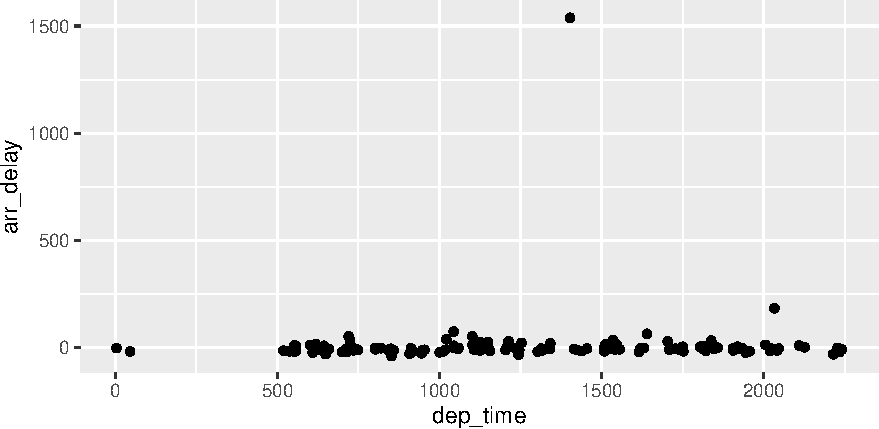
\includegraphics{my-thesis_files/figure-latex/march3plot-1.pdf}

\section{Additional resources}\label{additional-resources}

\begin{itemize}
\item
  \emph{Markdown} Cheatsheet - \url{https://github.com/adam-p/markdown-here/wiki/Markdown-Cheatsheet}
\item
  \emph{R Markdown}

  \begin{itemize}
  \tightlist
  \item
    Reference Guide - \url{https://www.rstudio.com/wp-content/uploads/2015/03/rmarkdown-reference.pdf}
  \item
    Cheatsheet - \url{https://github.com/rstudio/cheatsheets/raw/master/rmarkdown-2.0.pdf}
  \end{itemize}
\item
  \emph{RStudio IDE}

  \begin{itemize}
  \tightlist
  \item
    Cheatsheet - \url{https://github.com/rstudio/cheatsheets/raw/master/rstudio-ide.pdf}
  \item
    Official website - \url{https://rstudio.com/products/rstudio/}
  \end{itemize}
\item
  Introduction to \texttt{dplyr} - \url{https://cran.rstudio.com/web/packages/dplyr/vignettes/dplyr.html}
\item
  \texttt{ggplot2}

  \begin{itemize}
  \tightlist
  \item
    Documentation - \url{https://ggplot2.tidyverse.org/}
  \item
    Cheatsheet - \url{https://github.com/rstudio/cheatsheets/raw/master/data-visualization-2.1.pdf}
  \end{itemize}
\end{itemize}

\section{Mathematics and Science}\label{math-sci}

\section{Math}\label{math}

\TeX~is the best way to typeset mathematics. Donald Knuth designed \TeX~when he got frustrated at how long it was taking the typesetters to finish his book, which contained a lot of mathematics. One nice feature of \emph{R Markdown} is its ability to read LaTeX code directly.

If you are doing a thesis that will involve lots of math, you will want to read the following section which has been commented out. If you're not going to use math, skip over or delete this next commented section.

\section{Chemistry 101: Symbols}\label{chemistry-101-symbols}

Chemical formulas will look best if they are not italicized. Get around math mode's automatic italicizing in LaTeX by using the argument \texttt{\$\textbackslash{}mathrm\{formula\ here\}\$}, with your formula inside the curly brackets. (Notice the use of the backticks here which enclose text that acts as code.)

So, \(\mathrm{Fe_2^{2+}Cr_2O_4}\) is written \texttt{\$\textbackslash{}mathrm\{Fe\_2\^{}\{2+\}Cr\_2O\_4\}\$}.

\noindent Exponent or Superscript: \(\mathrm{O^-}\)

\noindent Subscript: \(\mathrm{CH_4}\)

To stack numbers or letters as in \(\mathrm{Fe_2^{2+}}\), the subscript is defined first, and then the superscript is defined.

\noindent Bullet: CuCl \(\bullet\) \(\mathrm{7H_{2}O}\)

\noindent Delta: \(\Delta\)

\noindent Reaction Arrows: \(\longrightarrow\) or \(\xrightarrow{solution}\)

\noindent Resonance Arrows: \(\leftrightarrow\)

\noindent Reversible Reaction Arrows: \(\rightleftharpoons\)

\subsection{Typesetting reactions}\label{typesetting-reactions}

You may wish to put your reaction in an equation environment, which means that LaTeX will place the reaction where it fits and will number the equations for you.

\begin{equation}
  \mathrm{C_6H_{12}O_6  + 6O_2} \longrightarrow \mathrm{6CO_2 + 6H_2O}
  \label{eq:reaction}
\end{equation}

We can reference this combustion of glucose reaction via Equation \eqref{eq:reaction}.

\subsection{Other examples of reactions}\label{other-examples-of-reactions}

\(\mathrm{NH_4Cl_{(s)}}\) \(\rightleftharpoons\) \(\mathrm{NH_{3(g)}+HCl_{(g)}}\)

\noindent \(\mathrm{MeCH_2Br + Mg}\) \(\xrightarrow[below]{above}\) \(\mathrm{MeCH_2\bullet Mg \bullet Br}\)

\section{Physics}\label{physics}

Many of the symbols you will need can be found on the math page \url{https://web.reed.edu/cis/help/latex/math.html} and the Comprehensive LaTeX Symbol Guide (\url{https://mirror.utexas.edu/ctan/info/symbols/comprehensive/symbols-letter.pdf}).

\section{Biology}\label{biology}

You will probably find the resources at \url{https://www.lecb.ncifcrf.gov/~toms/latex.html} helpful, particularly the links to bsts for various journals. You may also be interested in TeXShade for nucleotide typesetting (\url{https://homepages.uni-tuebingen.de/beitz/txe.html}). Be sure to read the proceeding chapter on graphics and tables.

\chapter[Vivianite as a phosphorus source in lake sediments: Importance of increased sulfate reduction on phosphorus mobilization]{\texorpdfstring{Vivianite as a phosphorus source in lake sediments: Importance of increased sulfate reduction on phosphorus mobilization\footnote{A modified version of this chapter was published as: van Kuppevelt H, Reitzel K, Hupfer M (2025) Vivianite as a phosphorus source in lake sediments: Importance of increased sulphate reduction on phosphorus mobilisation. J Soils Sediments. \url{https://doi.org/10.1007/s11368-025-03986-z}}}{Vivianite as a phosphorus source in lake sediments: Importance of increased sulfate reduction on phosphorus mobilization}}\label{vivianite-as-a-phosphorus-source-in-lake-sediments-importance-of-increased-sulfate-reduction-on-phosphorus-mobilization01-paper2}

\begin{figure}

{\centering 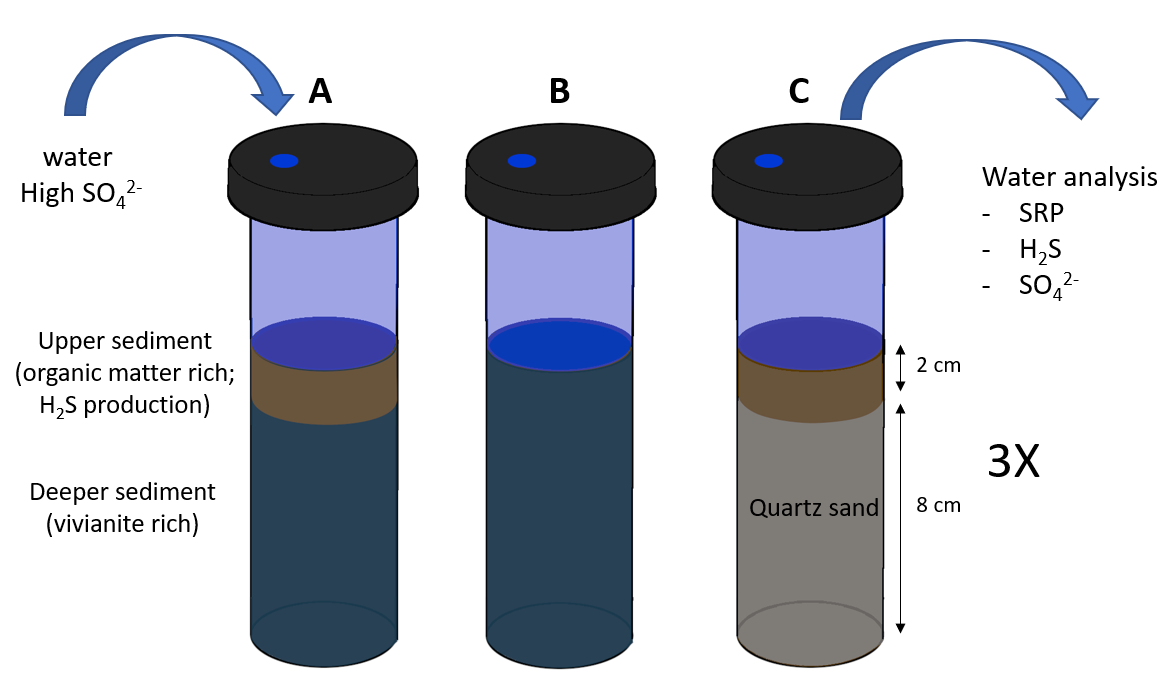
\includegraphics[width=0.7\linewidth]{figure/Setup_HS_Incubation_description} 

}

\caption{Graphic depicting the experimental mesocosm setup: organic matter-rich sediment (OM) was overlain on top of vivianite-rich sediment (Viv.). As control the two types of sediment were also incubated individually, with quartz sand (Qs) below the organic sediment to substitute the volume. At regular intervals, water samples were taken an analysed, and sulphate was replenished.}\label{fig:IncubationSetup}
\end{figure}

\section*{Abstract}\label{abstract}
\addcontentsline{toc}{section}{Abstract}

\noindent \textbf{Purpose}: Eutrophication of freshwater systems is primarily driven by excessive nutrient inputs, particularly phosphorus (P). While external nutrient control has been emphasized, the prediction and management of internal P loading from sedimentary sources remain complex. This study examines the role of vivianite (Fe(II)3(PO4)2·8H2O), a P-bearing mineral in anoxic sediments, in contributing to internal P release under sulfidic conditions.

\noindent \textbf{Materials and Methods}: A mesocosm experiment was conducted using sediment cores from Lake Arendsee, Germany. The cores were exposed to elevated sulfate concentrations to induce sulfate reduction, simulating anoxic and sulfidic conditions. Both water column chemistry and sediment solid-phase analyses were performed. P release from vivianite-rich sediments was monitored, along with changes in iron (Fe) mineral phases using sequential extraction and X-ray diffraction.

\noindent \textbf{Results and Discussion}: Increased sulfate reduction rates significantly mobilized P from vivianite-rich sediments, leading to elevated soluble reactive P levels in the water column. A marked decrease in vivianite content and an increase in sulfide-bound Fe species were observed in the sediments. These findings demonstrate that vivianite in Fe-rich sediments serves as an important internal P source under sulfidic conditions, exacerbating P release.

\noindent \textbf{Conclusions}: This study highlights the role of sulfur cycling in internal P loading and suggests that increased sulfate inputs may enhance eutrophication by mobilizing P from buried vivianite. Effective management of eutrophication should consider both external inputs and internal P sources like vivianite.

\section{Introduction}\label{introduction}

Eutrophication is a significant environmental issue that affects freshwater systems globally and is driven by an excess of nutrients in water bodies, resulting in excessive algal blooms, oxygen depletion, and diminished water quality \citep{Correll1998, Ansari2014}. Managing nutrient levels in water is crucial for the restoration of lake ecosystems and the prevention of further degradation. Phosphorus (P) often serves as a limiting factor for primary production and is a focal point for management interventions \citep{Azam2014, Tammeorg2024}. Despite concentrated efforts on controlling external sources of nutrients such as agricultural runoff and wastewater discharge, water quality targets remain unmet.

For instance, the EU's Water Framework Directive mandates member states to restore lakes within a relatively short time frame {[}WaterFrameworkDirective2000{]}. Consequently, contemporary lake management strategies aim to integrate both external and internal measures, with the latter focusing on mitigating the release of P from sediments into the water body \citep{Tammeorg2024}. Managing internal P release can accelerate the effectiveness of reducing external P sources and compensate for high external loads when external measures prove inadequate. A key strategy for internal control involves preventing the release of P from sequestered pools in sediments (burial P). Even after addressing external sources, the internal supply of P can perpetuate eutrophic conditions, especially when the water residence time is high \citep{Sondergaard2001, Wagner2020}. However, the processes and sources that drive P release from burial P are not yet fully understood.

The retention of P in sediments occurs through its binding to the solid phase via biological and chemical precipitation \citep{Boers1998, Parsons2017, OConnell2020}. Burial P pools accumulate in sediment following years of nutrient enrichment. The speciation of sediment P is highly dependent on lake conditions and undergoes significant changes during early diagenesis, where remobilization of labile forms of P occurs, whereas only the stable forms of solid-bound P are buried long-term \citep{Emerson1976, Boers1998}. Initially, the sedimentation of P incorporated into organic matter by primary producers is an important influx of P to lake sediments, especially in eutrophic lakes. However, the long-term burial of organic matter-bound P is constrained by remineralization processes in the sediment \citep{Boers1998}. Secondly, P can adsorb to iron (Fe) hydroxides \citep{Gunnars2002} and bind to organic matter to form organic Fe-P complexes \citep{Schwertmann1988}. The precipitation of these ferric Fe-bound P forms (Fe(III)-bound P) can be a major internal sink of P in lakes with naturally high Fe content \citep{Reitzel2005, Hupfer2008} or those artificially treated with Fe \citep{Kleeberg2012, Munch2024}. Under the reducing conditions induced by organic matter decomposition in the sediment, Fe(III) is reduced to Fe(II), leading to the release of bound P and preventing the long-term burial of Fe(III)-bound P. However, P can be sequestered long-term in the form of the Fe(II) mineral vivianite (Fe(II)₃(PO₄)₂·8H₂O) \citep{Rothe2016}, which has been identified as a major form of burial P in eutrophic, high-Fe, and non-sulfidic freshwater systems \citep{OConnell2015, Rothe2016, Dijkstra2018, Kubeneck2021}.

The role of sulfur (S) cycling in influencing Fe dynamics and internal P cycling has been recognized as crucial \citep{Kleeberg1997, Rozan2002, Wang2018, Heinrich2021}, including its impact on vivianite formation \citep{Rothe2015}. Sulfate (SO₄²⁻) is the dominant form of S in the water column but can be reduced to sulfide (S²⁻) by sulfate-reducing bacteria (SRB) in the sediment during decomposition processes. Sulfide readily binds to Fe, leading to the formation of Fe sulfides such as pyrite (FeS₂) and Fe monosulfide (FeS). This process effectively immobilizes Fe, removing it from the pool available to form Fe(III)--P or vivianite, thereby affecting the efficiency of P immobilization by Fe in sediments \citep{Heinrich2020}.

An increase in the sulfate reduction rate (SRR) can potentially remobilize the burial pools of Fe--P \citep{Roden1997, Katsev2006}. The SRR is influenced by the concentration of sulfate in the sulfate reduction zone, as well as other factors such as temperature \citep{Zhao2021, Han2023} and organic matter availability \citep{Chen2014, Zhao2019}. Several studies have reported a substantial increase in sediment P release following an increase in water sulfate concentrations in both laboratory experiments \citep{Zak2006, Baldwin2012, Chen2016, Zhou2022} and in situ studies \citep{Smolders1993, Lamers2002}. Over the past century, global freshwater sulfate concentrations have significantly increased because of human activities, remaining well above pre-industrial levels \citep{Kleeberg2014, Zak2021}.

The formation of vivianite in lake sediments is a focal point of ongoing research. Evidence of vivianite in older sediment strata underscores the significance of early diagenesis in its formation \citep{Dijkstra2018, Scholtysik2022}. This phenomenon has also been observed following Fe based treatments implemented for lake restoration \citep{Heinrich2021}. Prior research has identified the availability of Fe(III)--bound P \citep{Heinrich2020, Kubeneck2024}, redox fluctuations \citep{Parsons2017}, and microbial activity \citep{Cosmidis2014, Sanchez2015} as critical environmental factors influencing vivianite formation.

Although vivianite is redox stable and acts as a substantial P sink in anoxic sediments, its long-term stability is not well understood. Vivianite can incorporate significant amounts of P into its structure, contributing notably to the total phosphorus (TP) content in sediments; Rothe (2016) estimated that vivianite-bound P constituted approximately 50\% of TP at certain depths in Lake Arendsee \citep{Rothe2016}. Therefore, if vivianite-bound P pools exist within the sediment, their mobilization could sustain a prolonged release of internal P, exceeding duration estimated from traditional P sources such as Fe(III)--P \citep{Katsev2006}.

Scholars have hypothesized that an increase in sulphide production may lead to sustained P mobilization from buried vivianite by preferentially binding Fe \citep{Roden1997, Gachter2003, Katsev2006}. However, this process has not been directly demonstrated in situ, leaving its extent and significance for long-term P release uncertain. In a laboratory setting, Wilfert et al.~(2020) demonstrated that pure vivianite released up to 92\% of its P when exposed to sulfide \citep{Wilfert2020}. More recently, Kubeneck et al.~(2024) demonstrated that this process could also occur under natural pore water conditions by placing synthetic vivianite in mesh bags within the sulfidic sediments of an intertidal flat, resulting in a 30\% decrease in vivianite P \citep{Kubeneck2024}.

The present study aimed to further explore the dilapidation of vivianite within freshwater sediments and evaluate its potential contribution to P loading in the water column. This was accomplished by incubating authigenic vivianite in sediments from the sulfidic, dimictic Lake Arendsee in northern Germany, followed by monitoring the dissolution of vivianite and the subsequent release of P over time.
Reference figure 2 here \ref{fig:IncubationTimeseries}

\begin{figure}
\centering
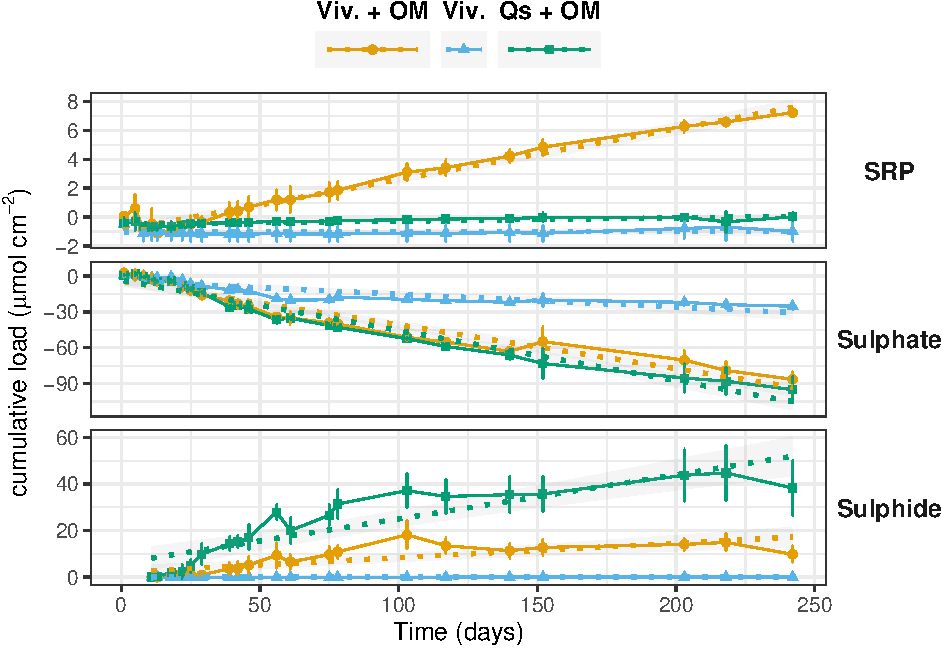
\includegraphics{my-thesis_files/figure-latex/IncubationTimeseries-1.pdf}
\caption{\label{fig:IncubationTimeseries}Time series of cumulative load of Soluble Reactive Phosphorus (SRP), sulphate, and sulphide to the water column from mesocosm during incubation over a period of approximately 250 days. The change of each species over time was fitted with a linear model, where the slope represents the release rate from the sediment to the water column, which values can be found in Table 2. Viv. + OM: cores with 8 cm of deep (30--35 cm sediment depth), vivianite-rich sediment overlain with 2 cm of sediment rich in organic matter. Viv.: 10 cm of vivianite-rich sediment. Qs + OM: 2 cm of organic matter-rich sediment, on top of 8 cm of quartz sand.}
\end{figure}

\section{Methods}\label{methods}

\subsection{Study Site}\label{study-site}

Sediment and water samples were collected from Lake Arendsee in northern Germany, located at 52°52'36.12''N, 11°29'12.12''E. Lake Arendsee is a dimictic lake, formed by salt karst processes, and has a relatively long water residence time of 50--60 years. The lake is primarily fed by groundwater and lacks natural drainage \citep{Meinikmann2015}. It reaches a maximum depth of 49.5 meters, an average depth of 29 meters, and covers a surface area of 5.14 km2. Since the 1960s, the lake has undergone significant eutrophication due to urban discharge from the city of Arendsee on the southern shore and drainage from nearby Lake Fauler \citep{Scharf1998}. P levels in the water column remain elevated due to ongoing groundwater P loading and the accumulation of P from historical inputs, exacerbated by the long water residence time \citep{Hupfer2019}.
In addition to high P concentrations (2023 yearly mean of 178 µg L-1; \url{https://www.igb-berlin.de/der-arendsee}), Lake Arendsee also contains considerable sulfate concentrations (61±7 mg L-1 in January 2023), originating from groundwater influenced by natural geological conditions, including gypsum in the catchment. The organic-rich top sediment layers exhibit significant sulfide production, leading to the formation of Fe sulfide with low total Fe content. In contrast, deeper in the sediment (below approximately 25 cm), the Fe content is much higher, and vivianite is a predominant Fe species \citep{Rothe2015, Scholtysik2022}.

\subsection{Sample collection}\label{sample-collection}

Surface water was collected into a 20 L plastic barrel, from which 10 L were filtered through pressure filtration (0.45 μm, cellulose acetate) to remove particulate matter, and then stored in 5 L canisters. Mixed sediment samples were obtained near the lake's deepest points and classified as organic matter-rich upper sediment (0--2 cm) and vivianite-rich deep sediment (30--35 cm). Sediment coring was performed using a UWITEC piston gravity corer with Plexiglas tubes measuring 60 cm in length and 6 cm in diameter. The cores were sectioned on-site, and the selected slices were carefully combined and stored in air-tight Ziplock bags, followed by vacuum sealing to minimize oxygen exposure. The samples were transported immediately to the laboratory and stored at 4 °C for less than a week before the commencement of the experiment. Approximately 2 L of vivianite-rich and 0.5 L of organic matter-rich sediments were collected.

\subsection{Sulphate reduction experiment}\label{sulphate-reduction-experiment}

The impact of sulfate reduction on vivianite in natural sediments was investigated by incubating the sediment in controlled mesocosms with added sulfate under anoxic conditions (Fig. \ref{fig:IncubationSetup}). The incubations were conducted in a climate chamber maintained at 12 °C. Unless otherwise noted, all water used in the experiments was sourced from Lake Arendsee and deoxygenated by bubbling with an N\textsubscript{2}/CO\textsubscript{2} mixture for a minimum of 6 h. Within a nitrogen-filled glove bag (Glas-Col 108D X-27-27H, O2 \textless1\%), sealed bags of sediment from Lake Arendsee were opened, transferred to a bucket, and vigorously stirred.
For the mesocosm setup, nine Plexiglas tubes---each 30 cm tall and 6 cm in diameter with sliding pistons at the bottom---were prepared in a glove bag for three sets of triplicate treatments. In the first treatment (Fig. \ref{fig:IncubationSetup}, A), tubes were filled with a combination of vivianite-rich and organic matter-rich sediments (Viv. + OM). In the second treatment (Fig. \ref{fig:IncubationSetup}, B), only vivianite-rich sediment was used (Viv.). In the third treatment (Fig. \ref{fig:IncubationSetup}, C), tubes contained only organic matter-rich sediment atop quartz sand, serving as an inert filler to equalise sediment and water column heights across treatments (Qs + OM; Fig. \ref{fig:IncubationSetup}).
Prior to the experiment, tubes designated for treatments Viv. and Viv. + OM were carefully filled with deep vivianite-rich sediment to a depth of 10 cm, ensuring no gas was trapped beneath the sediment. For the Qs + OM treatment, tubes were filled with equivalent volumes of quartz sand. Subsequently, the deoxygenated lake water was poured over the sediment to fill the tubes halfway. The tubes were stagnated overnight to allow the sediment to settle and create a uniform surface for the subsequent layer. The following day, the final sediment layer was added to the mesocosms for treatments Viv. + OM and Qs + OM. For each mesocosm, 60 mL of the upper sediment layer was transferred and allowed to settle at a well-defined sediment-water interface (SWI), after which the height of the water column above the SWI was measured.
Thereafter, all tubes were sealed with custom-made airtight caps equipped with stirring magnets and completely filled with anoxic surface water. The sulfate concentration in the overlying water was adjusted to 150 mg L\textsuperscript{-1} (1.6 mmol L\textsuperscript{-1}) by adding approximately 4 mL of a 10.01 g L\textsuperscript{-1} SO\textsubscript{4}\textsuperscript{2-} stock solution. Water samples were acquired immediately after setting up the mesocosms to confirm initial sulfate concentrations. The airtight caps ensured the maintenance of anoxic conditions throughout the 242-day incubation period. Sampling was conducted in a nitrogen atmosphere by flushing the glove bag before opening the caps. Water samples were taken at predetermined intervals, subsampled, and replenished with deoxygenated surface water. Sulfate levels were periodically adjusted to maintain a concentration of 150 mg L\textsuperscript{-1}. After the incubation, the sediment was analyzed to assess the variations in its solid-phase composition.

\subsection{Sample processing}\label{sample-processing}

At the end of the incubation period, the tubes were removed from the glove bag for subsequent processing. The caps were detached, and the final water samples were collected and subsampled before discarding the remaining water, leaving approximately 10 cm above the SWI. Despite air exposure after the removal of the caps and glove bag, the risk of oxygen affecting the sediment prior to slicing was minimal owing to the short duration of exposure compared to the time required for diffusive transport through the water column (hours versus days). The sediment was then sliced to determine the depth profiles of chemical composition and P speciation in the solid phase. To minimize oxygen exposure, sediment processing was conducted immediately and completed within 24 h. Additionally, the exposure was limited by storing the sediments in closed airtight containers, as oxidation can significantly alter P speciation in anoxic sediments \citep{Kraal2014}.
The upper 3 cm of the cores were sliced at 0.5 cm intervals, followed by two slices at 1 cm intervals, while deeper layers were sliced at 2 cm intervals down to a depth of 10 cm. The slices were carefully collected and homogenized. Mixed sediment sections were created by pooling equal weights from triplicate slices. This mixed sediment was stored in closed containers at 4 °C overnight, and subsamples were taken the following day for sequential extractions, analysis of dry weight (DW), and loss on ignition (LOI). After subsampling, the mixed sediment was frozen at -20 °C, then freeze dried and ground using an agate mortar and pestle. The dry, powdered sediments were stored in the dark at room temperature and later analysed for elemental and mineralogical composition.

\subsection{Chemical analysis}\label{chemical-analysis}

\subsubsection{Solid phase analysis}\label{solid-phase-analysis}

The DW and LOI of the sediment samples were determined by weighing approximately 1 g of subsamples, followed by drying at 105 °C for 24 h and combustion at 450 °C for 3 h, respectively. Elemental analysis of the dry sediment was conducted using reverse aqua regia digestion (DIN 38 414-S7, 1983). Approximately 70 mg of dried and ground sediment was digested in 2 mL of 37\% HCl and 6 mL of 65\% HNO3 in a high-pressure microwave oven (\#Prep-A, MLS 169 GmbH). Following dilution, element concentrations were measured by inductively coupled plasma optical emission spectrometry (ICP-OES).
To qualitatively assess the mineral composition and identify the presence of vivianite in dry sediment, powder X-ray diffraction (XRD) analyses were conducted. These analyses utilized a Bruker D2 Phaser equipped with a Cobalt X-ray source and an SSD160 detector. Each sample was analysed over a duration of 1 h, covering a range from 10° to 85° 2θ, with a step size of 0.014 2θ. The device settings included a rotating sample holder, a 1-mm fixed divergence slit, 2.5° primary and secondary Soller collimators, a fixed scatter screen at a 3 mm sample distance, and an Fe k-beta filter (2.5). The Bruker DIFFRAC.EVA software was employed for qualitative mineralogical analysis, with mineral identification achieved by comparing results with reference diffractograms from the Crystallography Open Database.

\subsubsection{Phosphorus Sequential Extraction}\label{phosphorus-sequential-extraction}

The P and Fe species in the sediment were determined using a sequential extraction protocol, which was originally developed by Psenner et al.~(1984) and later modified by Wang et al.~(2021) for vivianite extraction \citep{Psenner1984, Wang2021}. A precisely weighed 0.6 g of wet sediment was placed into 15 mL centrifuge tubes. The extraction process consisted of five steps (Table 1). Extracts were filtered, acidified, and analysed for P using the molybdenum blue method \citep{Murphy1962}. For the NaOH fraction, extracts were analysed both before and after digestion with K\textsubscript{2}S\textsubscript{2}O\textsubscript{8} to differentiate soluble reactive phosphorus (NaOH-SRP) from nonreactive phosphorus (NaOH-NRP). Specific fractions were designated for Fe analysis (BD-Fe and Bipy-Fe) using Atomic Absorption Spectroscopy (AAS; pinAAcle9001; PerkinElmer, Waltham, MA, USA).

\subsubsection{Dissolved elemental analysis}\label{dissolved-elemental-analysis}

Surface water samples were subdivided into three parts post-filtration (0.22 µm, 0.45 µm cellulose acetate). A 10 mL subsample was preserved with hydrochloric acid for P concentration analysis using the molybdate blue method (Murphy and Riley 1962). Sulfide concentrations in 2 mL subsamples were fixed with a 2\% zinc acetate solution (200 µL) and measured photometrically using the methylene blue method (Cline 1969). Sulfate concentrations were determined photometrically after filtering through a 0.22 µm cellulose acetate filter, using the BaSO4 colloid method \citep{Tabatabai1974}. Additionally, the elemental content (Fe, P, S, Mn, Ca, Al, and Ti) of the digested sediment was quantified using inductively coupled plasma optical emission spectroscopy (ICP-OES, iCAP 7000 series, Thermo Scientific).

\subsection{Data processing and statistical analysis}\label{data-processing-and-statistical-analysis}

Data analysis was conducted using R, and the detailed calculations are provided in the Supplementary Material. The release of P, sulfate, and sulfide from the sediment was determined by summing the changes in water column content at each time step, including any added sulfate stock. The variations in sediment composition were assessed by estimating the initial composition based on measurements of starting sediment compositions. This study utilized two types of sediments (Viv. + OM), with the estimated starting composition for each sediment slice derived from the concentrations of unchanged elements (Al, Ti, Fe, and Mn). Concentrations per volume and per surface area, integrated over the measured depths, were calculated from per-dry weight values by estimating the sediment bulk density from dry weight and loss on ignition (LOI) values \citep{Avnimelech2001}.
Per-surface area concentrations of dissolved species in the water column were also calculated to compare changes in the solid phase and water column, independent of variations in water column heights. The release rates were determined from concentration time series using the slope of the linear regression. Analysis of Variance (ANOVA) was employed to assess significant differences among the three treatments, followed by Tukey's honestly significant difference (HSD) test to identify the differences in specific treatment. The correlation between sulfate and sulfide concentrations in the water column was analysed using the Pearson correlation coefficient. The significant variations in sediment composition at all depths were tested using a paired t-test, with pairwise comparisons conducted at a 95\% family-wise confidence level.

\chapter{Paper 3}\label{paper3}

If we don't want Conclusion to have a chapter number next to it, we can add the \texttt{\{-\}} attribute.

\textbf{More info}

And here's some other random info: the first paragraph after a chapter title or section head \emph{shouldn't be} indented, because indents are to tell the reader that you're starting a new paragraph. Since that's obvious after a chapter or section title, proper typesetting doesn't add an indent there.

\chapter{Synthesis}\label{synthesis}

This thesis provides novel insights into the formation, composition, and stability of vivianite in intertidal
sediments. This chapter will begin with a summary of the key findings and their potential implications for the
role of vivianite in phosphorus (P) cycling in coastal sediments. The discussion will then extend to how the
presented findings may apply to various environmental systems and be relevant to other research fields. An
examination will follow, discussing how the developed methodology for in-situ studies in this thesis widens
our geochemical toolbox and opens various avenues to study in-situ Fe mineral transformation processes.
Additionally, this chapter suggests possible directions for future research.

\section{Summary and discussion}\label{summary-and-discussion}

\subsection{Vivianite stability under sulfidic conditions}\label{vivianite-stability-under-sulfidic-conditions}

The influence of sulphate reduction on phosphorus (P) mobilization i a process found in all aquatic systems, and has been observed in both marine and freshwater systems. Indeed, also in rivers this has been observed \citep{Zak2006}. There are a few key differences why the effect is different in lakes compared to rivers. In lakes, redox stratification often lead to more pronounced sulphate reduction. Secondly, the water residence time is much lower in rivers, and therefore inflow is relatively more important than sediment effects. However, for the same reason an increase of sulfate can be much larger in rivers \citep{Kommana2023}.
As for data on the proportion of phosphorus associated with higher sulphate levels in lakes and rivers, it is important to make a difference between the short and long term. There are many studies that have examined this relationship in the short term in specific systems \citep[e.g.][]{Roden1997, Chen2016, Zhao2021} . However, as far as I'm aware there is no recent review study. The importance of sulfur on the long term P retention is much more difficult to quantify, although there is some modelling evidence \citep{Katsev2006} suggesting it may play a major role.

\subsection{Methodological considerations}\label{methodological-considerations}

Bipyridine extraction.
Sediment peeper.
Mössbauer, Xanes
Synthetic vs natural vivianite.

\section{Conclusions and outlook}\label{conclusions-and-outlook}

\subsection{Implications for freshwater management}\label{implications-for-freshwater-management}

Diagnostics.
Fe treatment.
Sulfate management.
Dredging.

\subsection{Relevance to other fields}\label{relevance-to-other-fields}

The RecaP project aims to look in a transdisciplinary fashion at the P challenge, in order to come to a holistic transformation towards sustainable P use. It is therefore crucial to place the implications of this study in a broader context.

\subsubsection{further up the P value chain}\label{further-up-the-p-value-chain}

Stakeholder engagement. Farmer and industry responsibility sulfur mitigation. Reuse of vivianite P from lakes. Lake health as indicator for P recycling success.

\subsubsection{Climate change and biodiversity loss}\label{climate-change-and-biodiversity-loss}

Lakes as biodiversity hotspots and widespread effects of eutrophication

\subsubsection{Paleosedimentology and diagenesis}\label{paleosedimentology-and-diagenesis}

It is interesting to put the relative fluxes of P from antropogenic sources to the geological cycle.
Post- depositional alteration of sediment record \citep{Dijkstra2018} Apatite as main P mineral in geoleogical cycle\citep{Zhao2024}

\subsection{Future research}\label{future-research}

Mössbauer.
Find case study where legacy vivianite P is mobilized.
Investigate the potential of sulfate management for P control.
Develop robust model for predicting Fe treatment efficacy.

\appendix

\chapter{The First Appendix}\label{the-first-appendix}
\addcontentsline{toc}{chapter}{References}
\renewcommand\bibname{References}
\bibliography{bib/thesis.bib}

% -----------------------------------------------
% OPTIONAL LISTS OF FIGURES/TABLES
% -----------------------------------------------
  \listoffigures
  \clearpage

  \listoftables
  \clearpage

\end{document}
